\documentclass[11pt]{article}

% Loading packages
\usepackage[margin=1in]{geometry}
\usepackage{array}
\usepackage{color}
\usepackage{amsmath}
\usepackage{amsthm}
\usepackage{amsfonts}
\usepackage{hyperref}
\usepackage{listings}
\usepackage{natbib}
\usepackage{url}
\usepackage{graphicx}
\usepackage{graphics}
\usepackage[position=t,singlelinecheck=off,justification=centering,labelformat=empty]{subfig}
\usepackage{fancyhdr}
\usepackage{rotating}
\usepackage{multirow}
\usepackage[usenames,dvipsnames]{xcolor}
\usepackage{sectsty}
\usepackage{titlesec}
\usepackage{booktabs}
\usepackage{datetime}
\usepackage{tikz}
\usepackage{type1cm}
\usepackage{lettrine}
\usepackage{comment}
\usepackage{morefloats}
\usepackage{longtable}
\usepackage{psfrag}
\usepackage{changepage}
\usepackage{fancyhdr}



\parskip 1pc
\setlength{\parindent}{0pt}
%\renewcommand\familydefault{\sfdefault}
%\renewcommand{\thesection}{\large\arabic{section}}
%\allsectionsfont{\large}
\settimeformat{ampmtime}
\mmddyyyydate

\lstloadlanguages{TeX}
\lstset{backgroundcolor=\color{white},
numbers=left, basicstyle=\footnotesize\ttfamily,
numbersep=2pt, stepnumber=1}

\definecolor{linkcolor}{rgb}{0,0,0.50}
\setcitestyle{authoryear, round, semicolon, aysep={},yysep={;},notesep={,}}
\hypersetup{
    bookmarks=true,                 % show bookmarks bar?
    unicode=false,                  % non-Latin characters in bookmarks
    pdftoolbar=true,                % show toolbar?
    pdfmenubar=true,                % show menu?
    pdffitwindow=true,              % window fit to page when opened
    pdfstartview={FitH},            % fits the width of the page to the window
    pdftitle={},                    % title
    pdfauthor={BPS team},           % author
    pdfnewwindow=true,              % links in new window
    colorlinks=true,                % false: boxed links; true: colored links
    linkcolor=blue,                 % color of internal links
    citecolor=black,                % color of links to bibliography
    filecolor=magenta,              % color of file links
    urlcolor=blue,                  % color of external links
    breaklinks=true
}
%\fancyfoot{}
\pagestyle{fancy}

\setcitestyle{authoryear, round, semicolon, aysep={},yysep={;},notesep={,}}

\newcommand{\HRULE}[1]{\color{#1}{\rule{2pc}{.018in}}}
\definecolor{gold}{rgb}{0.85,.66,0}
\definecolor{blue}{rgb}{0,0,1}

\def\results{S:/trainings/LaTeX/results}
\def\bs{\begin{sideways}}
\def\es{\end{sideways}}


\title{\LaTeX{} Training}
\author{Jamie Fogel \\
        Research Assistant \\
        Federal Reserve Bank of Boston \\
        \href{mailto:james.fogel@bos.frb.org}{james.fogel@bos.frb.org}
        }
\date{August, 2013}

\begin{document}


\fancyfoot[RO, RE]{\hyperlink{contents}{Back to Table of Contents}}
\renewcommand{\headrulewidth}{0pt}
\lhead{\LaTeX{} Training}
%\chead{\leftmark}
\rhead{Section \thesection}
\lfoot{Jamie Fogel}
\cfoot{\thepage}

\maketitle

\input{S:/example.tex}


\begin{abstract}
    The goal of this training session is to familiarize you with \LaTeX{}, explain to you when and why you should use \LaTeX{}, and to provide some simple examples to help you get started. \LaTeX{} is a typesetting program which allows users to create documents (usually pdfs) with more ease and flexibility that word processors, such as Word. The primary advantage of Word is its low startup cost. Just about anyone can open Word, start typing, and produce something acceptable. This is fine when your document will be almost entirely text, but adding equations, section numbers, citations, tables, and figures can be a total mess in Word. \LaTeX{} provides the user much more control over how all of these features appear in the finished document and turns out to be much easier than Word with a little practice. I do not expect you to be proficient in \LaTeX{} after this training session, but my goal is for you to know how to get started and to provide enough examples of code that you will be able to accomplish most of your tasks by piecing together and slightly altering pieces of my code.
\end{abstract}

\clearpage

\hypertarget{contents}{}
\tableofcontents

\section[Alternative Title for Section on Sections and Subsections]{Sections and Subsections}

Creating automatically numbered sections and subsections in \LaTeX{} is easy! To create a section, simply include
\begin{verbatim}
    \section{Section Name}
\end{verbatim}

\subsection{How to create a subsection}
\begin{verbatim}
     \subsection{Subsection Name}
\end{verbatim}

\subsubsection{You can even create subsubsections!}
\begin{verbatim}
    \subsubsection{Subsubsection Name}
\end{verbatim}


\section{Pretty Equations}

Suppose we want to write a set of equations. A good way of doing this is to use the align environment, shown below. We use ``\&='' rather than ``='' in order to align the equals signs on different lines. If we did not want to align the equals signs, we would simply write ``=''.

\begin{align}
    \tilde{E} &= \bar{e}(E+U+N)\\
    \tilde{U} &= \frac{\bar{e}\bar{u}(E+U+N)}{1-\bar{u}}\\
    \tilde{N} &= (E+U+N)(1-\bar{e}-\frac{\bar{e}\bar{u}}{1-\bar{u}})
\end{align}

Now, suppose we want to omit the equation numbers. We do this be replace ``align'' with ``align*'', shown below:

\begin{align*}
    \tilde{E} &= \bar{e}(E+U+N)\\
    \tilde{U} &= \frac{\bar{e}\bar{u}(E+U+N)}{1-\bar{u}}\\
    \tilde{N} &= (E+U+N)(1-\bar{e}-\frac{\bar{e}\bar{u}}{1-\bar{u}})
\end{align*}

\section{Figures}

First, let's create a simple figure. In Stata, I plotted labor force flows from employed to unemployed in eps format and saved it as ``S:/trainings/LaTeX/results/EE.eps.'' If all we want is a very simple figure, we simply tell \LaTeX{} to open a figure, reference the saved image fill we want to include in the figure, and finally end the figure. The code on the left produces the table on the right.\footnote{The actual code I used to put the figure code next to the figure, which you will see if you look at the underlying \TeX{} file, is a little more complicated.}

\begin{figure}[h!]
    \begin{minipage}[c]{.45\textwidth}
        \centering
        \begin{verbatim}
\begin{figure}[h!]
   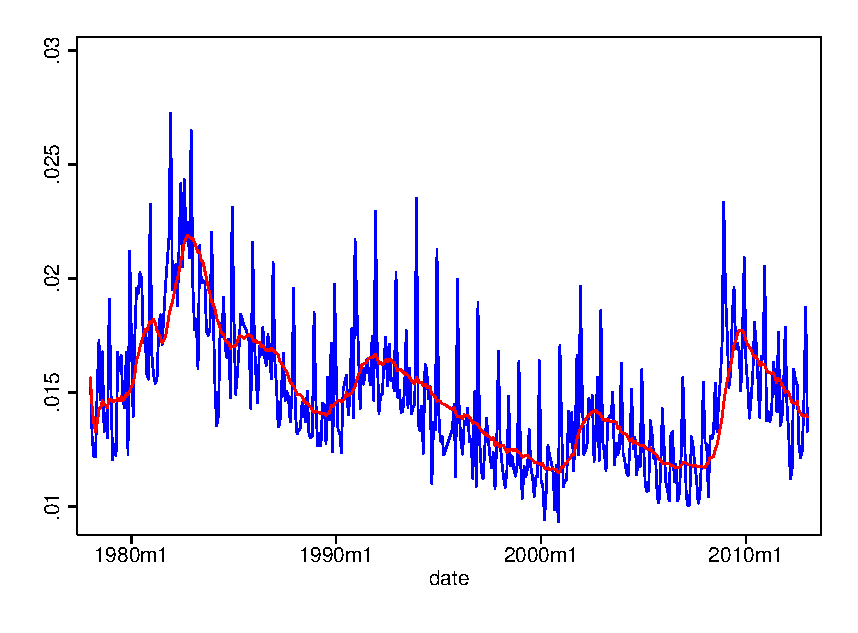
\includegraphics{\results/EU.eps}
\end{figure}
        \end{verbatim}
    \end{minipage}
    \begin{minipage}[c]{.45\textwidth}
        \centering
        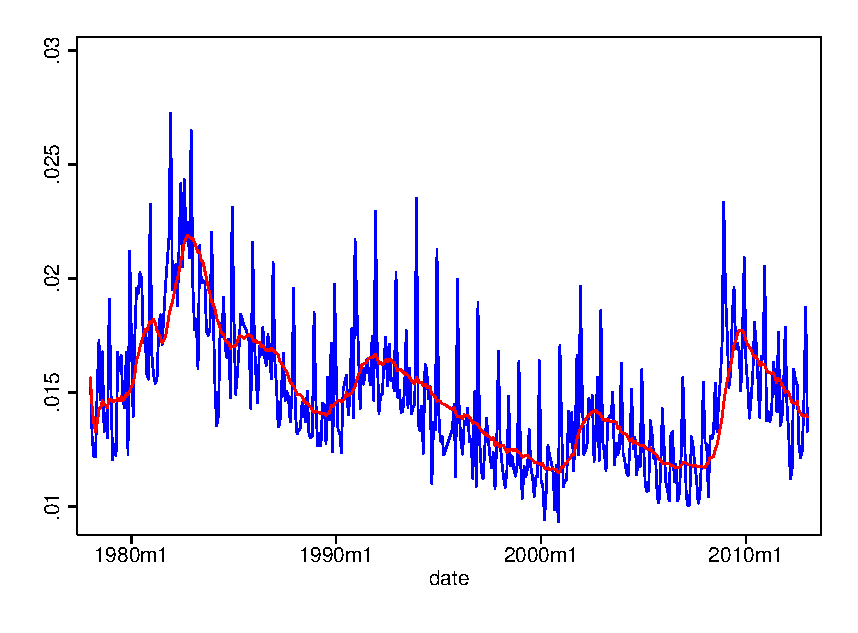
\includegraphics[width=.95\textwidth]{\results/EU.eps}
    \end{minipage}
\end{figure}

This is a very simple figure. In reality, you are likely to include at least a caption and footnote in your figure. To do this, just add a few lines to the code above:
\begin{verbatim}
\begin{figure}[h!]
    \centering
    \caption{Employed to Unemployed Flows}
    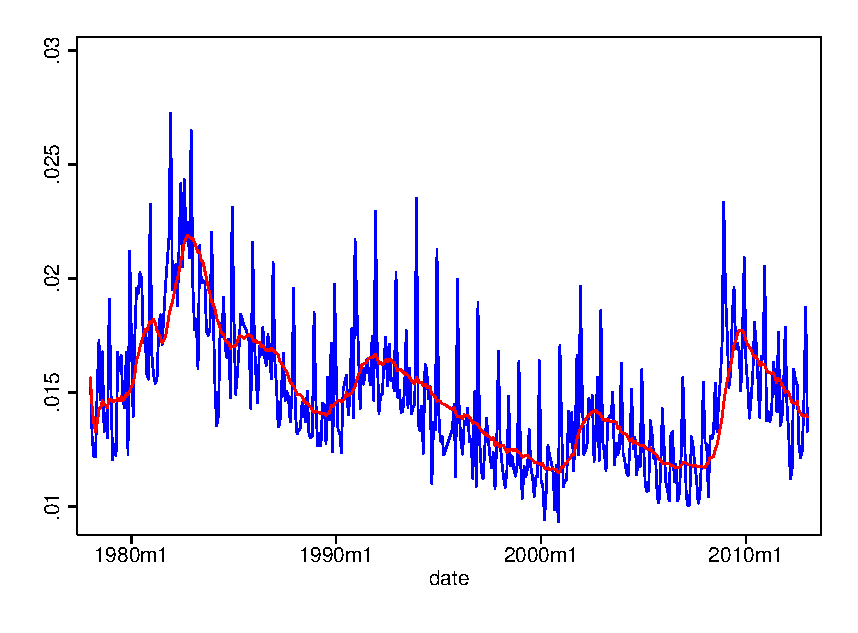
\includegraphics[width=.95\textwidth]{\results/EU.eps}\\
    \flushleft \footnotesize Flows in blue; 12-month moving average in red.\\ Source: BLS and Author's Calculations
\end{figure}
\end{verbatim}


\begin{figure}[h!]
        \centering
        \caption{Employed to Unemployed Flows}
        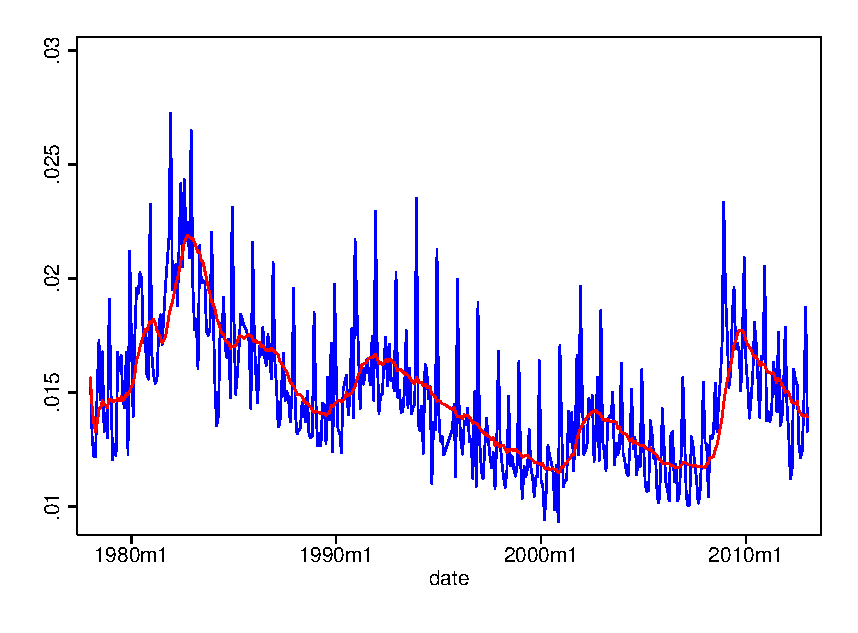
\includegraphics[width=.95\textwidth]{\results/EU.eps}\\
        \flushleft \footnotesize Flows in blue; 12-month moving average in red.\\ Source: BLS and Author's Calculations
\end{figure}


Now, let's combine multiple graphs into one figure. I do not provide the underlying code here because it is a little bit more complicated than the simple examples above, but when you look at it you will notice that it does little more than combine and several elements of the code used to produce the simple figures above. Figure \ref{multipletable} is wider than it is long, so it would be nice to rotate it and make more efficient use of the entire page. As I show in figure \ref{sidewaystable}, this is trivially easy and only requires us to change
\begin{verbatim}
\begin{figure}[h!]
    ...
\end{figure}
\end{verbatim}
to
\begin{verbatim}
\begin{sidewaysfigure}[h!]
    ...
\end{sidewaysfigure}
\end{verbatim}

\begin{figure}[h!]
        \caption{Labor Force Flows}
        \centering
        \subfloat[EE]{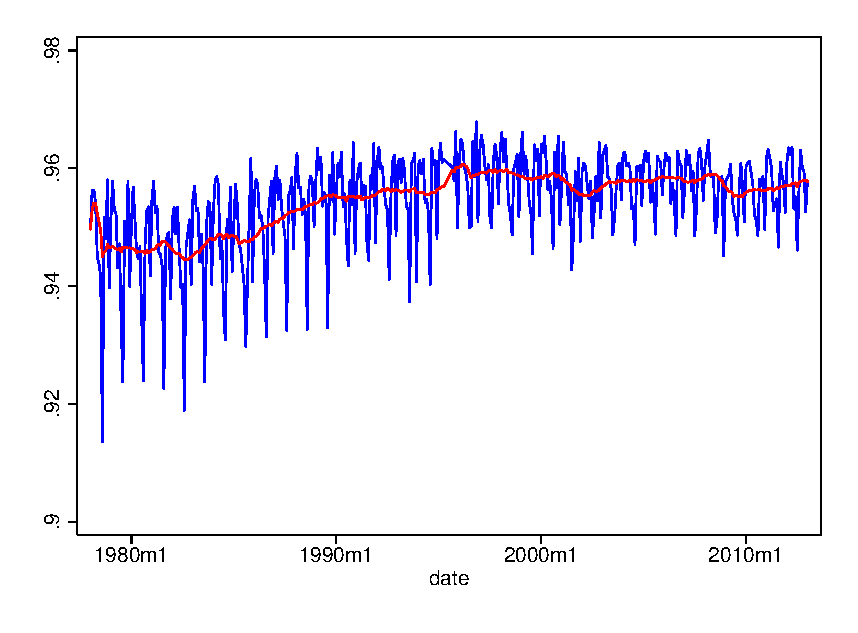
\includegraphics[width=.33\textwidth]{\results/EE.eps}}
        \subfloat[EU]{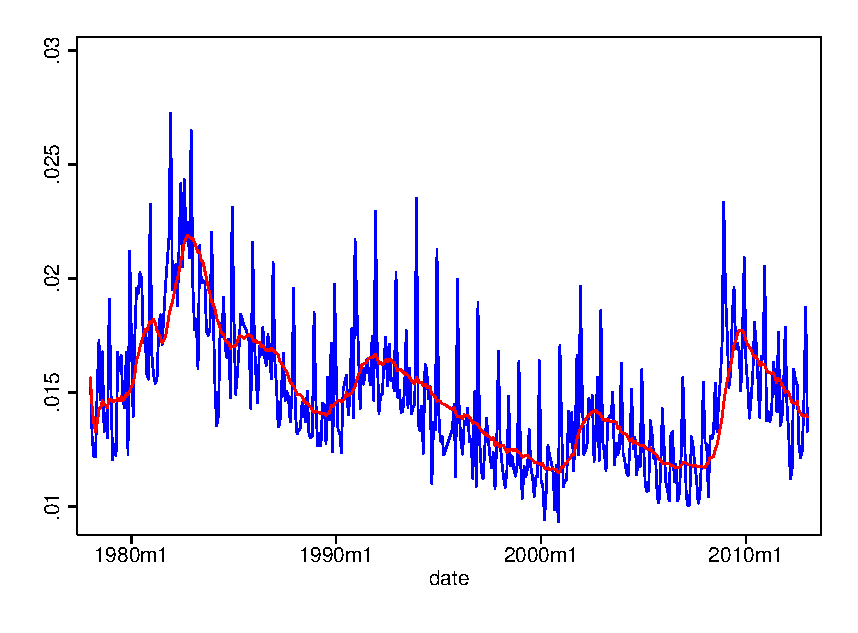
\includegraphics[width=.33\textwidth]{\results/EU.eps}}
        \subfloat[EN]{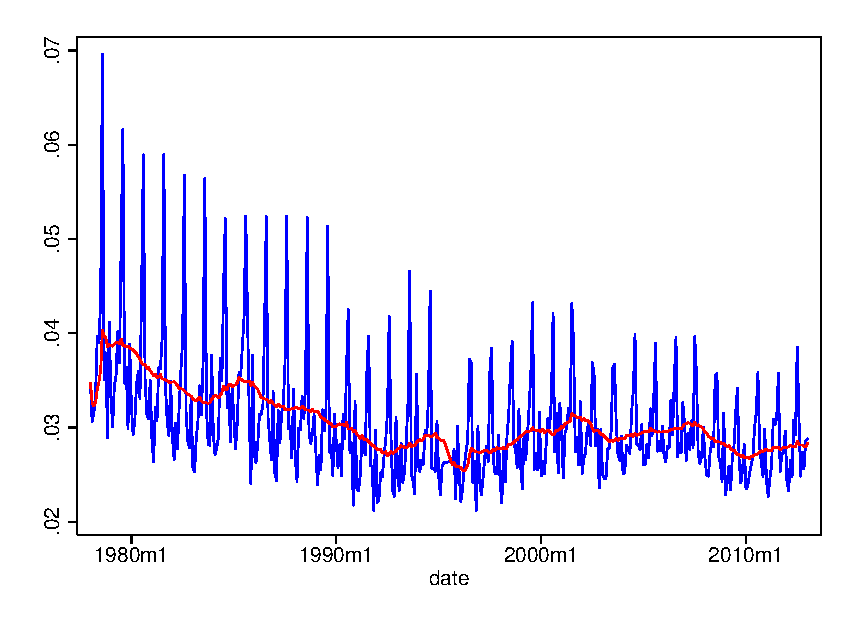
\includegraphics[width=.33\textwidth]{\results/EN.eps}}\\
        \subfloat[UE]{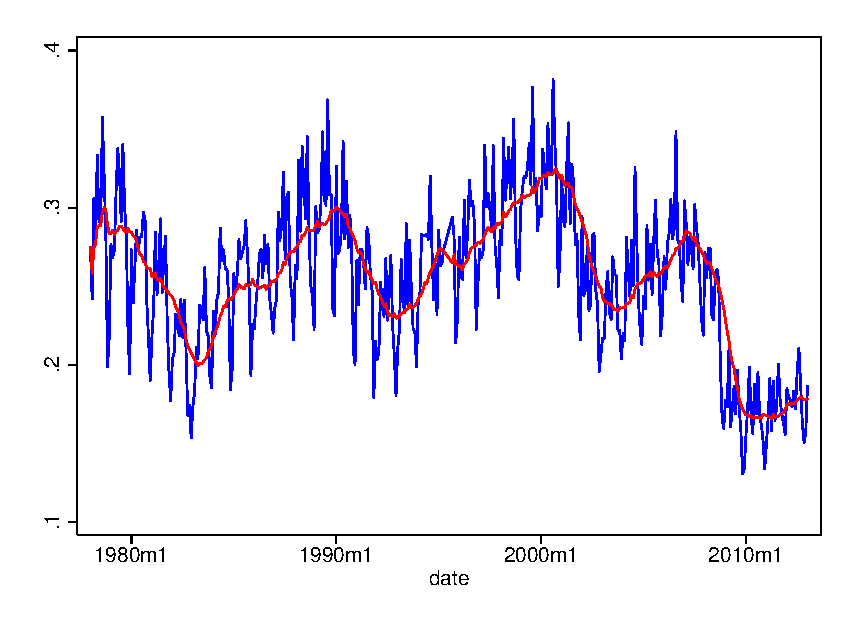
\includegraphics[width=.33\textwidth]{\results/UE.eps}}
        \subfloat[UU]{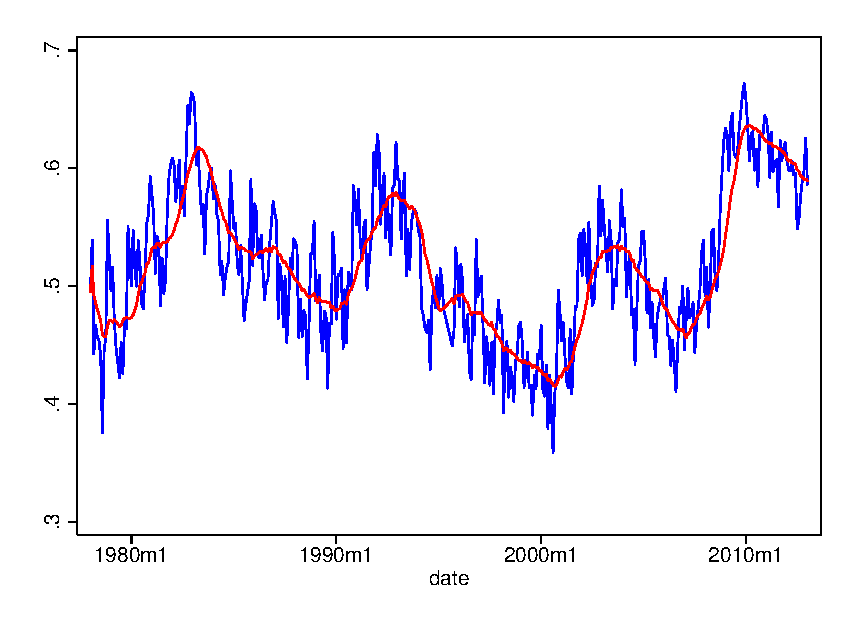
\includegraphics[width=.33\textwidth]{\results/UU.eps}}
        \subfloat[UN]{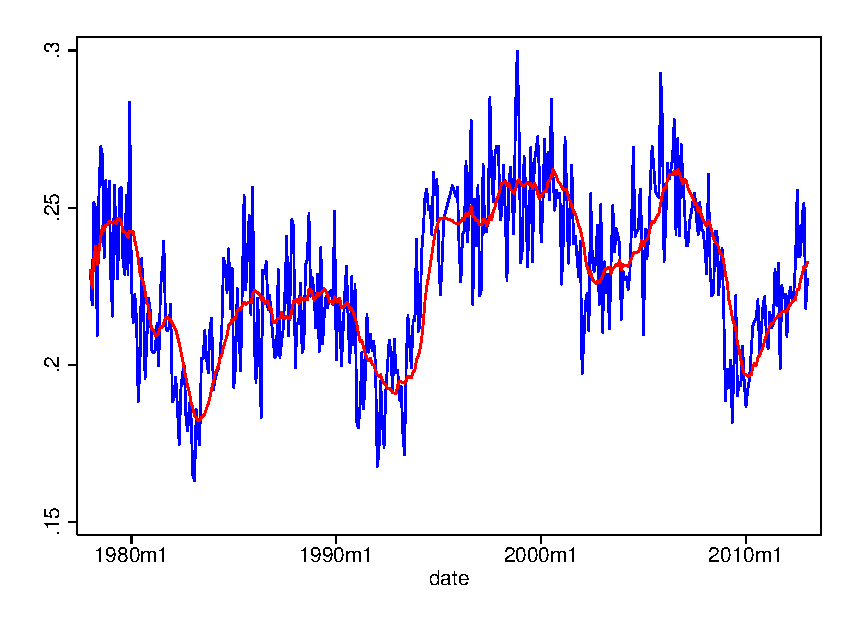
\includegraphics[width=.33\textwidth]{\results/UN.eps}}\\
        \subfloat[NE]{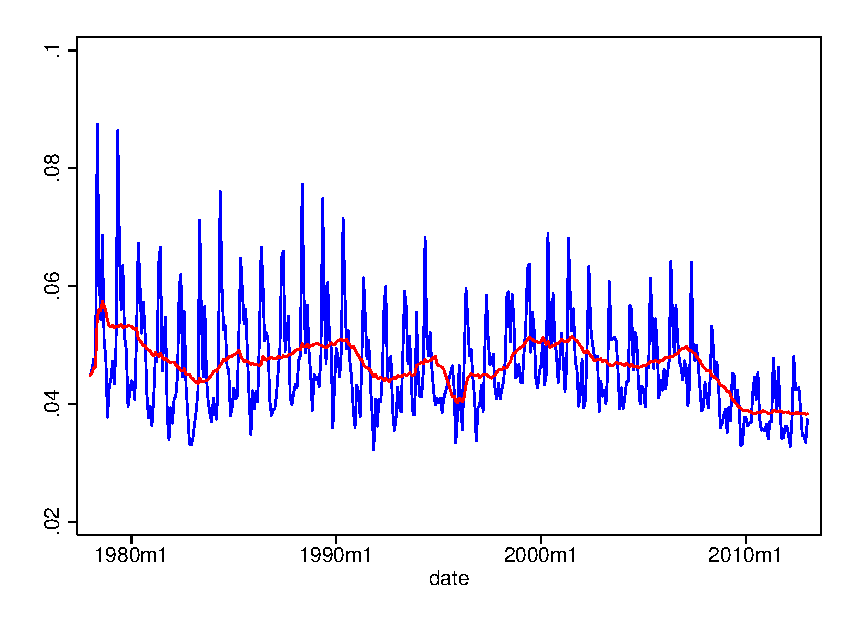
\includegraphics[width=.33\textwidth]{\results/NE.eps}}
        \subfloat[NU]{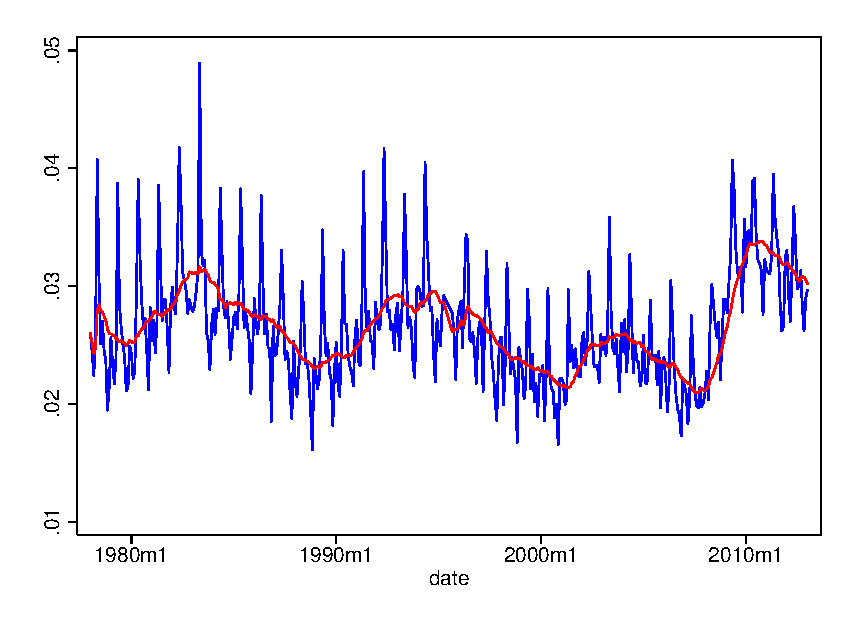
\includegraphics[width=.33\textwidth]{\results/NU.eps}}
        \subfloat[NN]{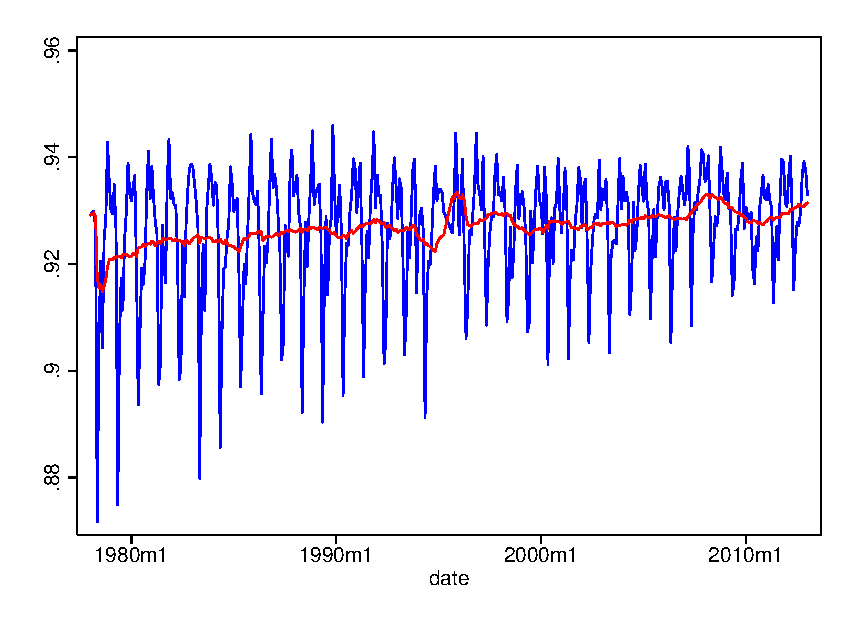
\includegraphics[width=.33\textwidth]{\results/NN.eps}}\\
        \flushleft \footnotesize Flows in blue; 12-month moving average in red.\\ Source: BLS and Author's Calculations
        \label{multipletable}
\end{figure}

\begin{sidewaysfigure}[h!]
        \caption{Labor Force Flows}
        \centering
        \subfloat[EE]{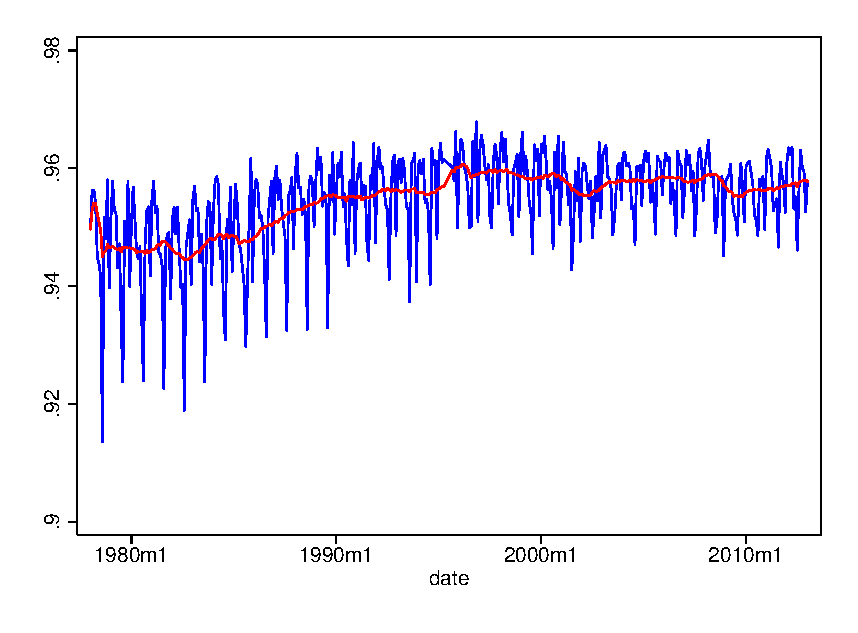
\includegraphics[width=.33\textwidth]{\results/EE.eps}}
        \subfloat[EU]{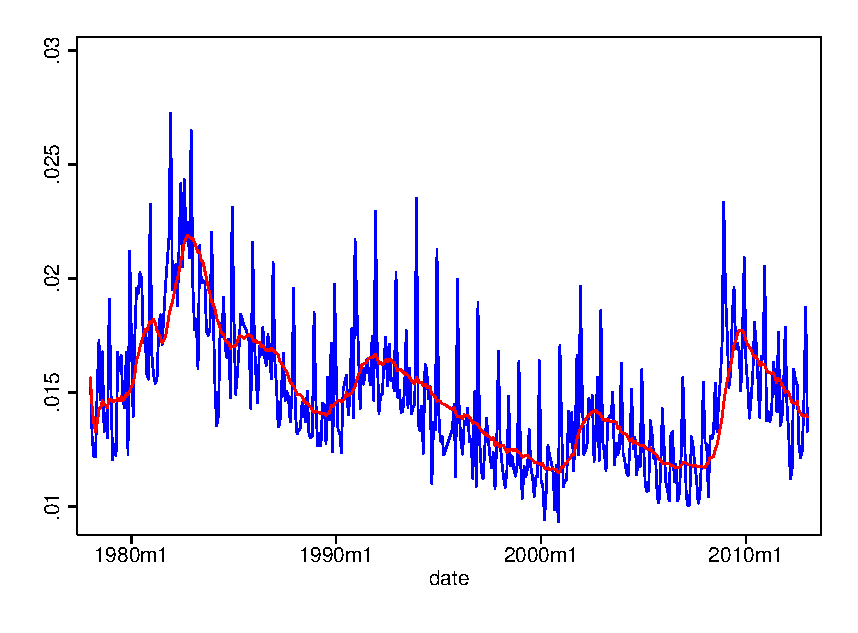
\includegraphics[width=.33\textwidth]{\results/EU.eps}}
        \subfloat[EN]{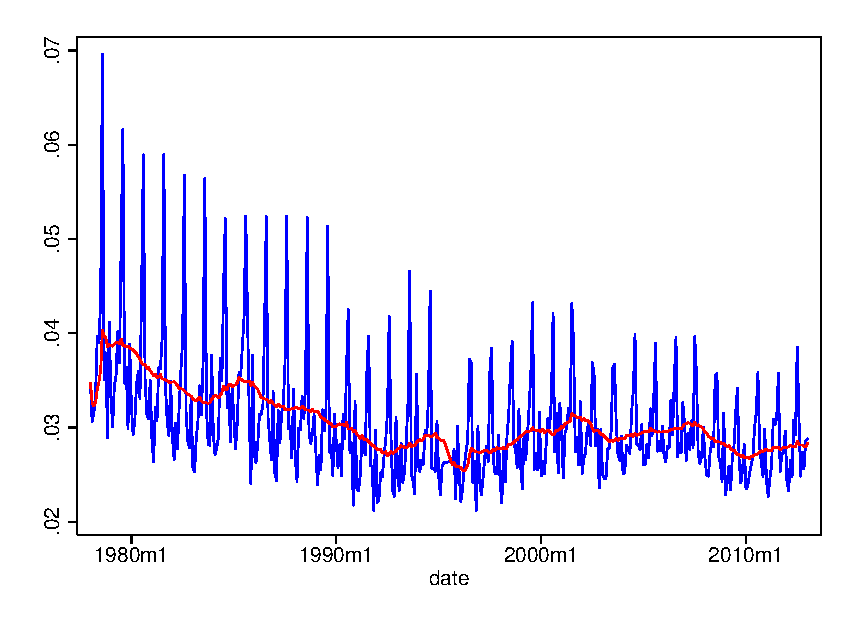
\includegraphics[width=.33\textwidth]{\results/EN.eps}}\\
        \subfloat[UE]{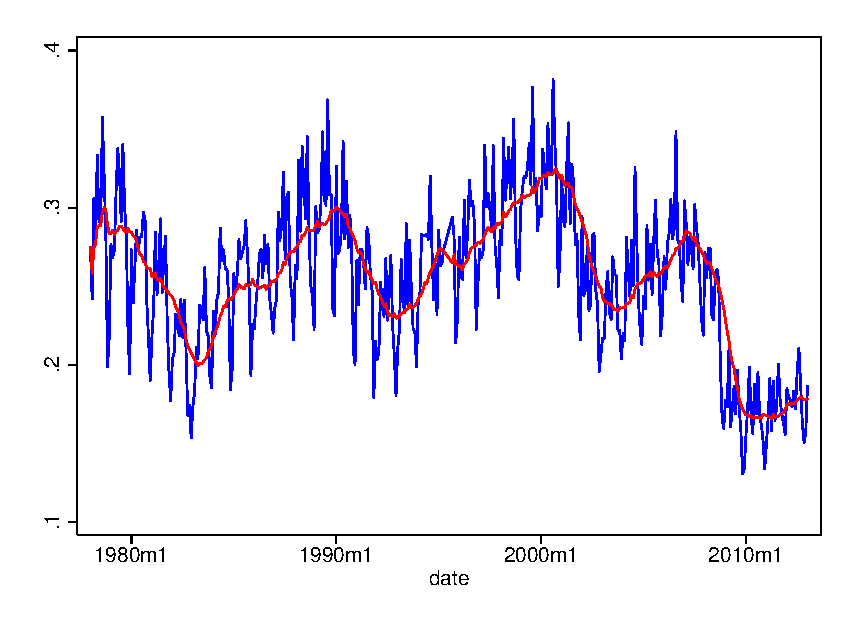
\includegraphics[width=.33\textwidth]{\results/UE.eps}}
        \subfloat[UU]{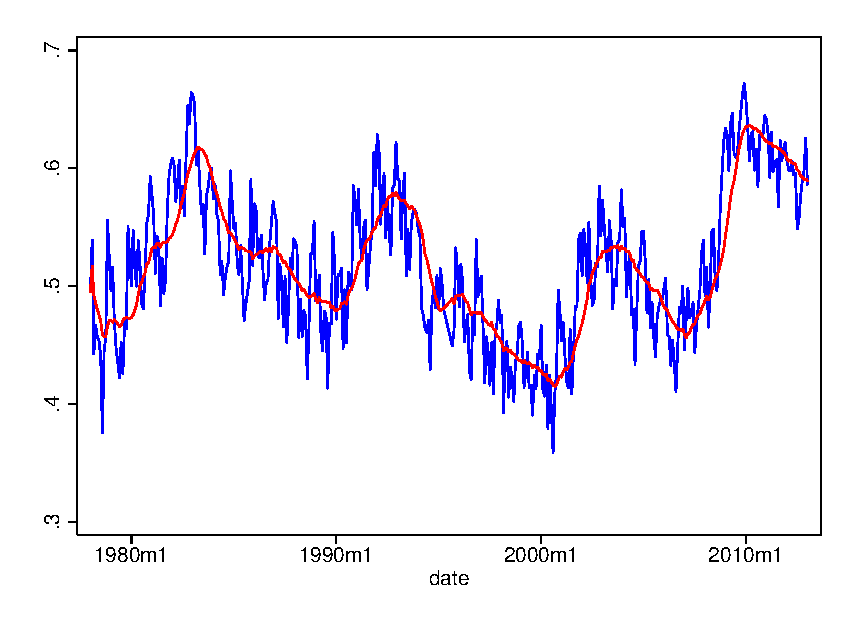
\includegraphics[width=.33\textwidth]{\results/UU.eps}}
        \subfloat[UN]{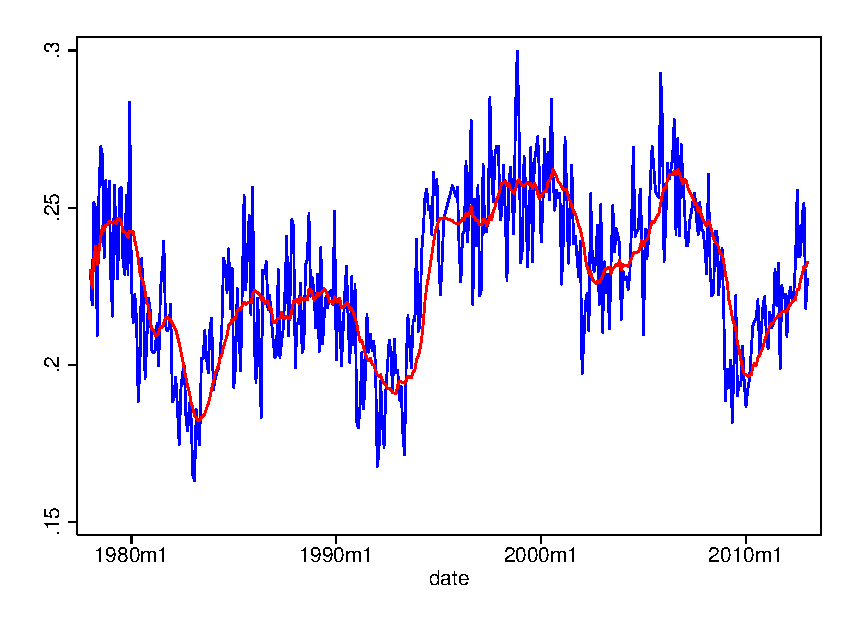
\includegraphics[width=.33\textwidth]{\results/UN.eps}}\\
        \subfloat[NE]{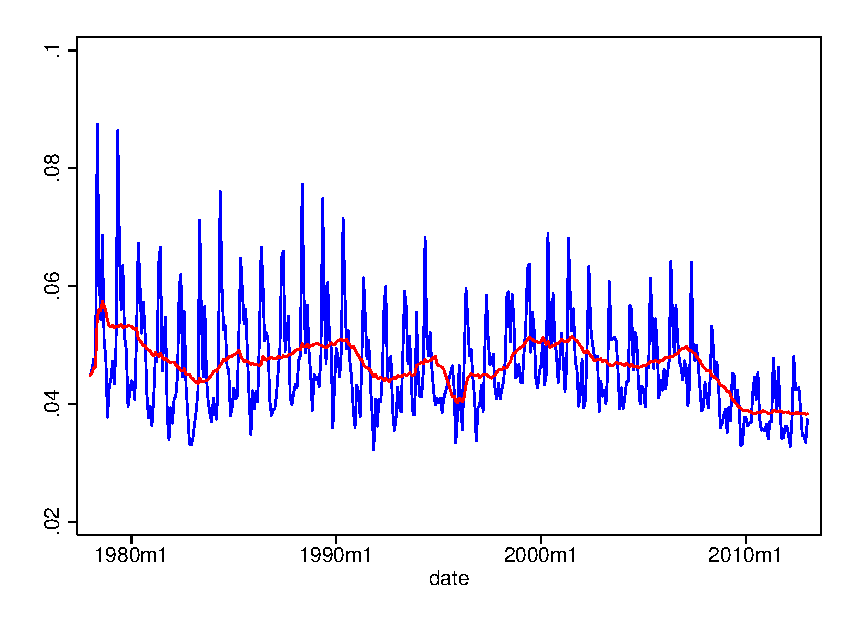
\includegraphics[width=.33\textwidth]{\results/NE.eps}}
        \subfloat[NU]{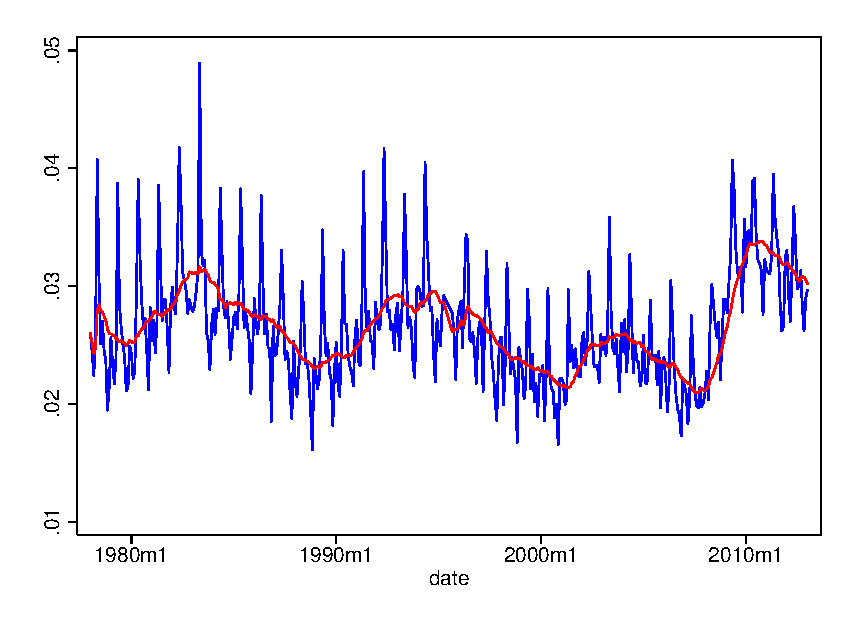
\includegraphics[width=.33\textwidth]{\results/NU.eps}}
        \subfloat[NN]{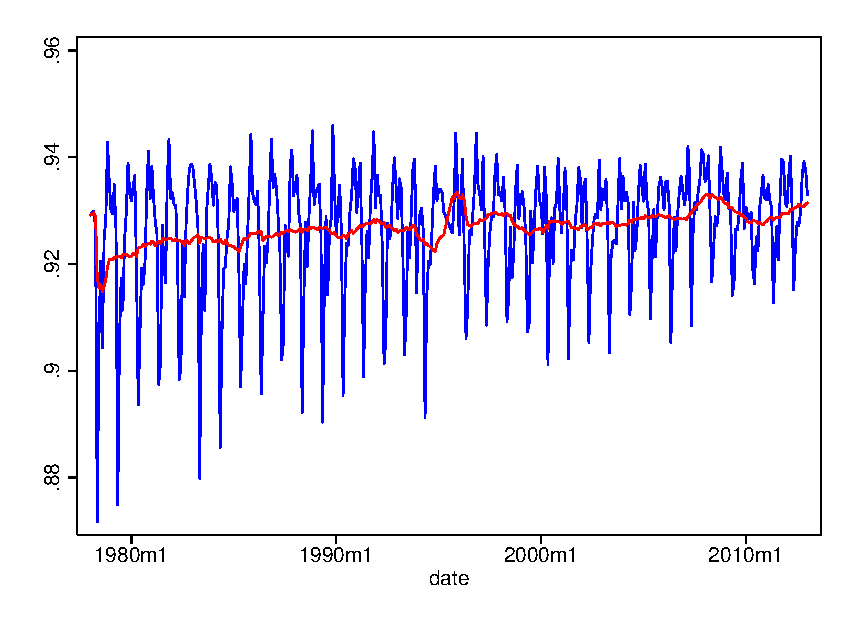
\includegraphics[width=.33\textwidth]{\results/NN.eps}}\\
        \flushleft \footnotesize Flows in blue; 12-month moving average in red.\\ Source: BLS and Author's Calculations
        \label{sidewaysfigure}
\end{sidewaysfigure}

\clearpage

Alternatively, we could have created the exact same figure using \lstinline=foreach= loops:
\begin{lstlisting}
\begin{sidewaysfigure}[h!]
        \caption{Labor Force Flows}
        \centering
        \foreach \F in {EE,EU,EN}{
            \subfloat[\F]{\includegraphics[width=.33\textwidth]{\results/\F.eps}}
        } \\
        \foreach \F in {UE,UU,UN}{
            \subfloat[\F]{\includegraphics[width=.33\textwidth]{\results/\F.eps}}
        } \\
        \foreach \F in {NE,NU,NN}{
            \subfloat[\F]{\includegraphics[width=.33\textwidth]{\results/\F.eps}}
        } \\
        \flushleft \footnotesize Flows in blue; 12-month moving average in red.\\ Source: BLS and Author's Calculations
        \label{sidewaysfigure2}
\end{sidewaysfigure}
\end{lstlisting}
\begin{sidewaysfigure}[h!]
        \caption{Labor Force Flows}
        \centering
        \foreach \F in {EE,EU,EN}{
            \subfloat[\F]{\includegraphics[width=.33\textwidth]{\results/\F.eps}}
        } \\
        \foreach \F in {UE,UU,UN}{
            \subfloat[\F]{\includegraphics[width=.33\textwidth]{\results/\F.eps}}
        } \\
        \foreach \F in {NE,NU,NN}{
            \subfloat[\F]{\includegraphics[width=.33\textwidth]{\results/\F.eps}}
        } \\
        \flushleft \footnotesize Flows in blue; 12-month moving average in red.\\ 
        Source: BLS and Author's Calculations
        \label{sidewaysfigure2}
\end{sidewaysfigure}

\clearpage

\section{Hyperlinks}

\LaTeX{} enables users to easily add hyperlinks to their documents. This can be very useful for a number of reasons. A simple and obvious use is creating links to websites. For example, \url{http://en.wikibooks.org/wiki/LaTeX/Hyperlinks} is a great source for more information on hyperlinks. Including the whole url in the text can be a bit clunky, however, so you may want to add a description to the link. The same website can be accessed by \href{http://en.wikibooks.org/wiki/LaTeX/Hyperlinks}{clicking here}. You can insert email links. You can email me by \href{mailto:james.fogel@bos.frb.org}{clicking here} or clicking on my email address, \href{mailto:james.fogel@bos.frb.org}{james.fogel@bos.frb.org}. All the links you see here are highlighted in blue, however you can change the color by editing the \begin{verbatim}\hypersetup{ ... }\end{verbatim} command in the document preamble or anywhere else in the document. For example, I can change the email link to green\hypersetup{urlcolor=green}: \href{mailto:james.fogel@bos.frb.org}{james.fogel@bos.frb.org}; or black: \hypersetup{urlcolor=black} \href{mailto:james.fogel@bos.frb.org}{james.fogel@bos.frb.org}. Black is especially useful when dealing with citations, which may be hyperlinks to the relevant line in the references section but don't want the hyperlink to be obvious to the reader.

\section{Tips and tricks}

\begin{itemize}
    \item Sometimes \LaTeX{} will fail to compile and you will be totally at a loss for what the problem is. Try deleting all of the auxiliary files created in the same directory as your .tex file and recompile your document. Sometimes this will solve the problem.
\end{itemize}

\section{Text Formatting}

Changing the font size \url{https://engineering.purdue.edu/ECN/Support/KB/Docs/LaTeXChangingTheFont}

\end{document}
